\chapter{Supporting Materials}

\begin{figure}
\centering
\includegraphics[width=\textwidth]{Figures/mutationanalysisbreakpoints.pdf}
\caption[Structural variant and mutation rates of HER2+ and TNBC PDX]
	{\small
	\textbf{Structural variant and mutation rates of HER2+ and TNBC PDX.}
	    \textbf{(a)} Distribution over copy number
breakpoints/cell as a function of generation for left: TNBC, right: HER2+
\textbf{(b)} Clone specific distributions over copy number breakpoints/cell, coloured by fitness coefficients for left: TNBC, right: HER2+
\textbf{(c)} Clone specific distributions over point mutations/cell, coloured by fitness coefficients for left:TNBC, right:HER2+
}
    \label{fig:Umutationanalysisbreakpoints}
    \end{figure}


















\begin{figure}
\centering
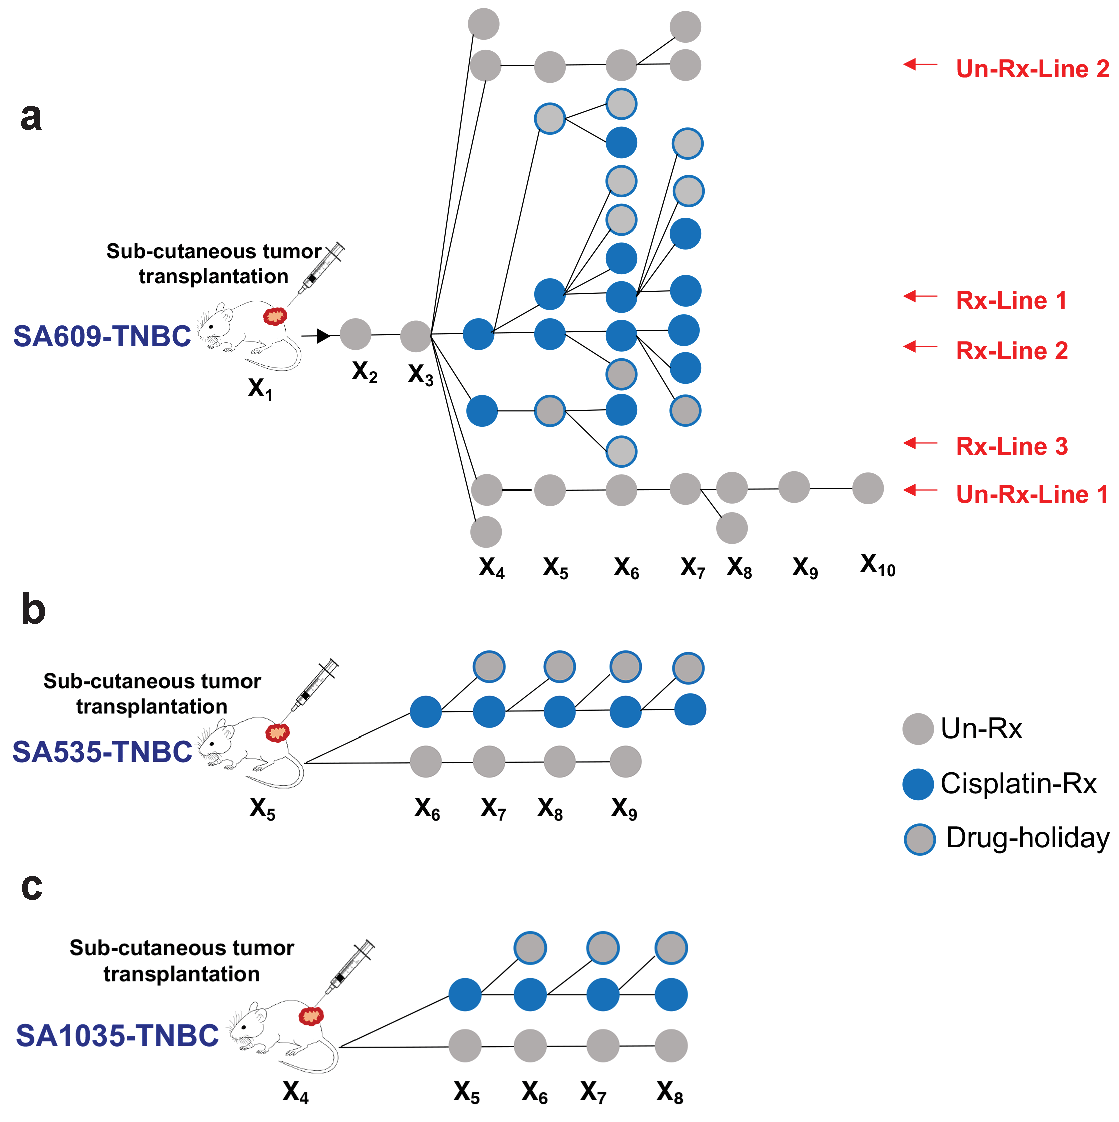
\includegraphics[width=\textwidth]{Figures/treatedtimeseriesmanuscript.pdf}
	
\caption[TNBC PDX timeseries clonal dynamics under drug perturbations]
	{\small
	\textbf{TNBC PDX timeseries showing timepoint nodes used for single cell whole genome sequencing}
	     All nodes representing each PDX tumour were digested to acquire genomes of single cells (~200-600 cells/tumor). Extra replicate tumors at each time point are not shown in the diagram (n=2-4). Grey circles represent un-treated, blue represents Cisplatin treated and grey with blue outline presents drug-holiday samples  \textbf{(a)} SA609-TNBC time series with replicates. DLP+ collected starting from X1 to X10 (Un-Rx line 1). Top grey branch indicating Un-Rx line 2. The middle three branches are cisplatin treated time series replicate branches  \textbf{(b)} SA535-TNBC  showing the tumor nodes taken for DLP+ starting from X5 untreated  \textbf{(c)} SA1035-TNBC  showing the tumor nodes taken for DLP+ starting from X 4 untreated.}
	\label{fig:Untreated timeseries growth curves only}
\end{figure}




\begin{figure}
\centering
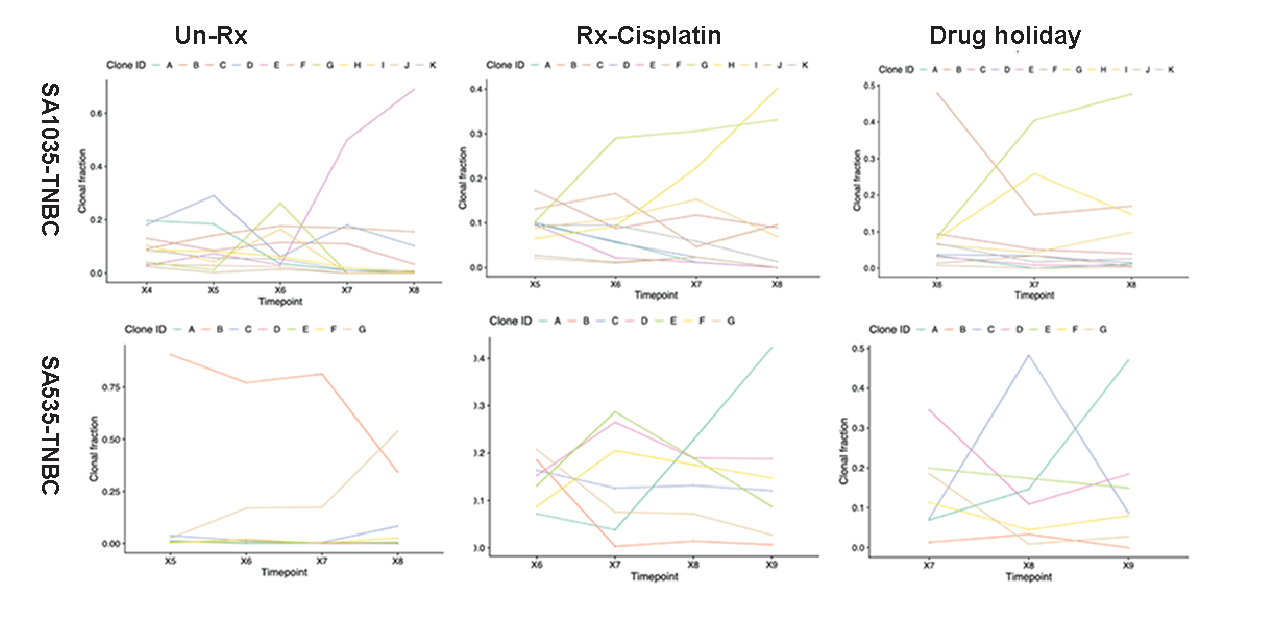
\includegraphics[width=\textwidth]{Figures/drugholidaysamples.pdf}
	
\caption[TNBC-SA609 PDX reproducible clonal dynamics with and without treatment]
	{\small
\textbf{Observed trajectories including drug-holiday samples.}
Panels showing line trajectories of clonal behaviour over time in two additional TNBC all three conditions. Fitness reversal in drug holiday samples of SA1035 and SA535 were not very prominent as compare to SA609. Horizontal axis representing the timepoints of each generation and vertical axis shows clonal fractions.
	}
	\label{fig:Untreated timeseries growth curves only}
\end{figure}






\begin{figure}
\centering
\includegraphics[width=\textwidth]{Figures/SA1035_AllCyclesCisplatin.pdf}
	
\caption[Tumor growth curves from SA1035 TNBC PDX]
	{\small
\textbf{Tumor growth curves from SA1035 TNBC PDX.}
Tumour response curves in each cycle of cisplatin treatment in SA1035 TNBC PDX. The vertical axis on right indicates tumor status and on left shows tumor volume. Horizontal axis presents days post measurable tumor.
}
	\label{fig:Untreated timeseries growth curves only}
\end{figure}
